\begin{figure}[!ht]
	\centering
	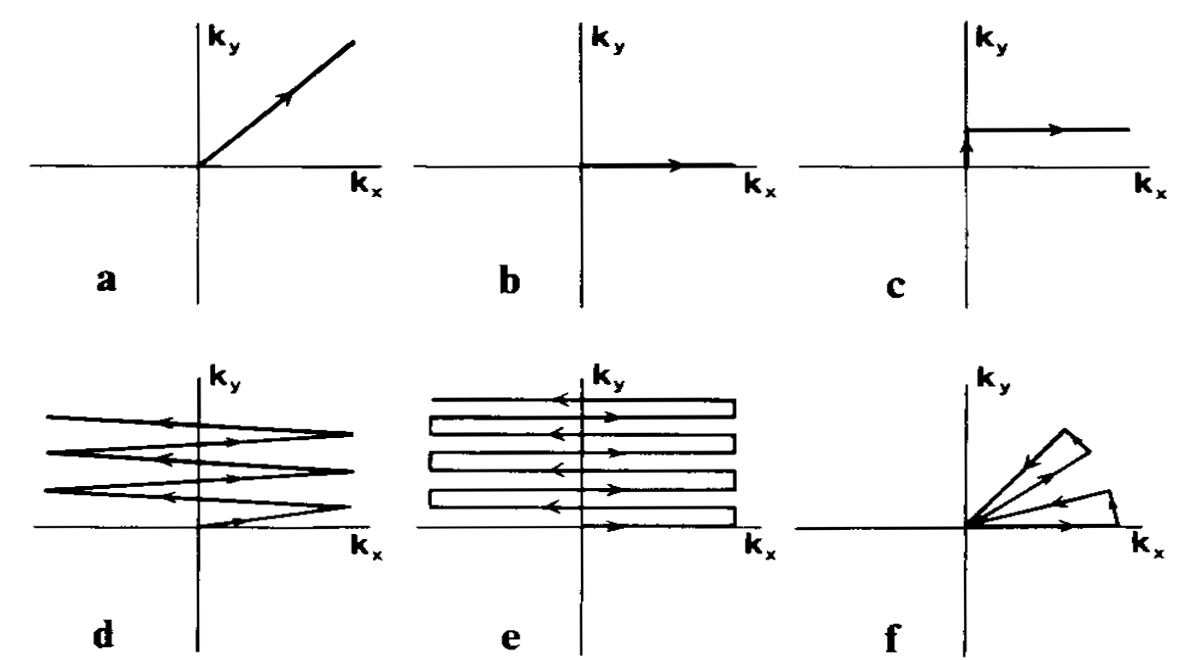
\includegraphics[width=0.6\textwidth, clip=true]{./Chapters/01_Introduction/Images/Kspace}
	\caption{Simple $k$-space representations \cite{Ljunggren1983} for projection imaging (a), line scanning (b), Fourier imaging (c), EPI (d), modified EPI (e), and modified projection imaging (f). The $k$-space is a helpful way with which MRI acquisition can be illustrated.}
	\label{fig:kspace}
\end{figure}